\documentclass[11pt]{article}

\newcommand{\cnum}{CS188}
\newcommand{\ced}{Winter 2017}
\newcommand{\ctitle}[3]{\title{\vspace{-0.5in}\cnum, \ced\\Problem Set #1: #2\\Due #3}}
\usepackage{enumitem}
\usepackage{graphicx}
\newcommand{\solution}[1]{{{\color{blue}{\bf Solution:} {#1}}}}
\usepackage[usenames,dvipsnames,svgnames,table,hyperref]{xcolor}

\renewcommand*{\theenumi}{\alph{enumi}}
\renewcommand*\labelenumi{(\theenumi)}
\renewcommand*{\theenumii}{\roman{enumii}}
\renewcommand*\labelenumii{\theenumii.}


\begin{document}
\ctitle{2}{programming}{2/16,2017}
\author{}
\date{}
\maketitle
\vspace{-0.75in}

\section{Problem 4}
\begin{enumerate}
\item Problem 4a
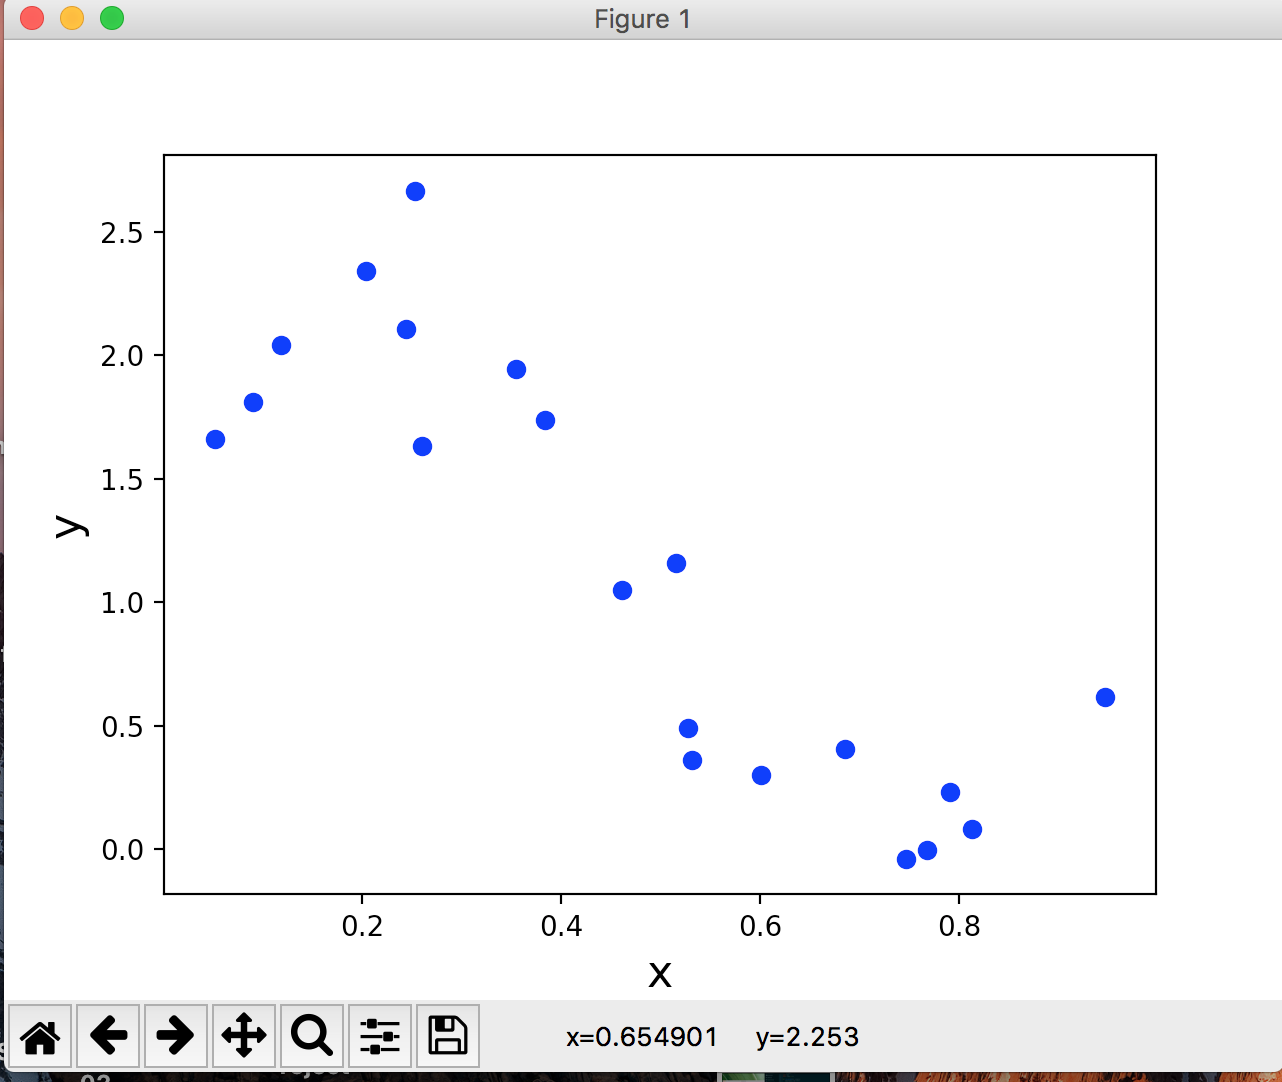
\includegraphics[scale=0.5]{ps21.png}
\solution{
In general, we see that the data does appear roughly linear, but with a noticeable amount of noise. For the most part, we see that y decreases with x, but there are exceptions, such as y increasing with x for x in teh range of 0 to 0.3. From the very limited data that we have, I would guess that a linear regression could be appropriate since the data appears roughly linear. A polynomial regression may also be appropriate since the data resemble a curved plot.
}

\vspace{1cm}
\item Problem 4b

\solution{I changed the code to do the tasks.}
\vspace{1cm}
\item Problem 4c
\solution{I changed the code to do the tasks.}
\vspace{1cm}

\item Problem 4d \newline{} Cost refers to the final value of the obj. func \newline{}
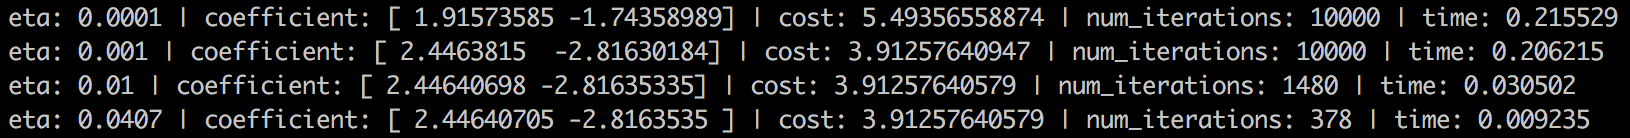
\includegraphics[scale=0.55]{PS22Real.png}
\solution{The coefficients are almost exactly the same (up to the 3rd decimal place), besides the ones generated by the smallest eta, which did not reach as low of a cost as the others had. For etas of 0.0001 and 0.001, the algorithm iterated for the same number of times (the maximum, 10k), but for the eta of 0.0001, we didn't get as low of a cost. Next, the eta of 0.01 took 1480 iterations (about 10x less than the previous etas), while the eta of 0.0407 took 378 iterations, so it converged much quicker. I used python's time.clock() to also time each function.}
\vspace{1cm}
\item Problem 4e \newline{}
\solution{
the closed form solution is: [ 2.44640709 -2.81635359]
the coefficients are almost exactly the same as what we got when we did GD with 0.001. 0.01, and 0.0407 etas, but different from the 0.0001 eta. 
\newline{}
for the closed form solution, the cost was 3.91257640579, which is almost exactly what we got we did GD with 0.001. 0.01, and 0.0407 etas, but different from the 0.0001 eta.
\newline{}
Since there's no sense of iteration in the closed form solution algorithm, I used python's time.clock() to get a sense of the running speed. It ran in 0.000271 on my computer. The fastest GD ran in 0.009 seconds, so this closed form solution is about 45x faster. I think this is because the dataset was relatively small and numpy has very efficient matrix operations implemented in optimized C. For very large datasets, gradient descent may be more appropriate. 
}
\vspace{1cm}
\item problem 4f
\solution{With the learning rate that's a function of the iterations, the fit gd algorithm took 0.227652 seconds to converge, but it iterated until the limited (10k). \newline{}
The full data for the learning rate as a function is: \newline{}
iters: 10000,time: 0.227652,cost: 3.91257642432
decay coefs: [ 2.44634965 -2.81623746]
}

\vspace{1cm}
\item problem 4g
\solution{i wrote the code for this.}

\vspace{1cm}
\item problem 4h
\solution{
RMSE, or root mean squared error, measures how good the fit is, while J measures how strong the correlation is. So since RMSE indicates how good our fit is, this may be a preferable metric because we want to know how well our learned parameters are fitting to the dataset, this can be more indicative of a model's quality than knowing about correlation.
}

\vspace{1cm}
\item problem 4i
\newline{}
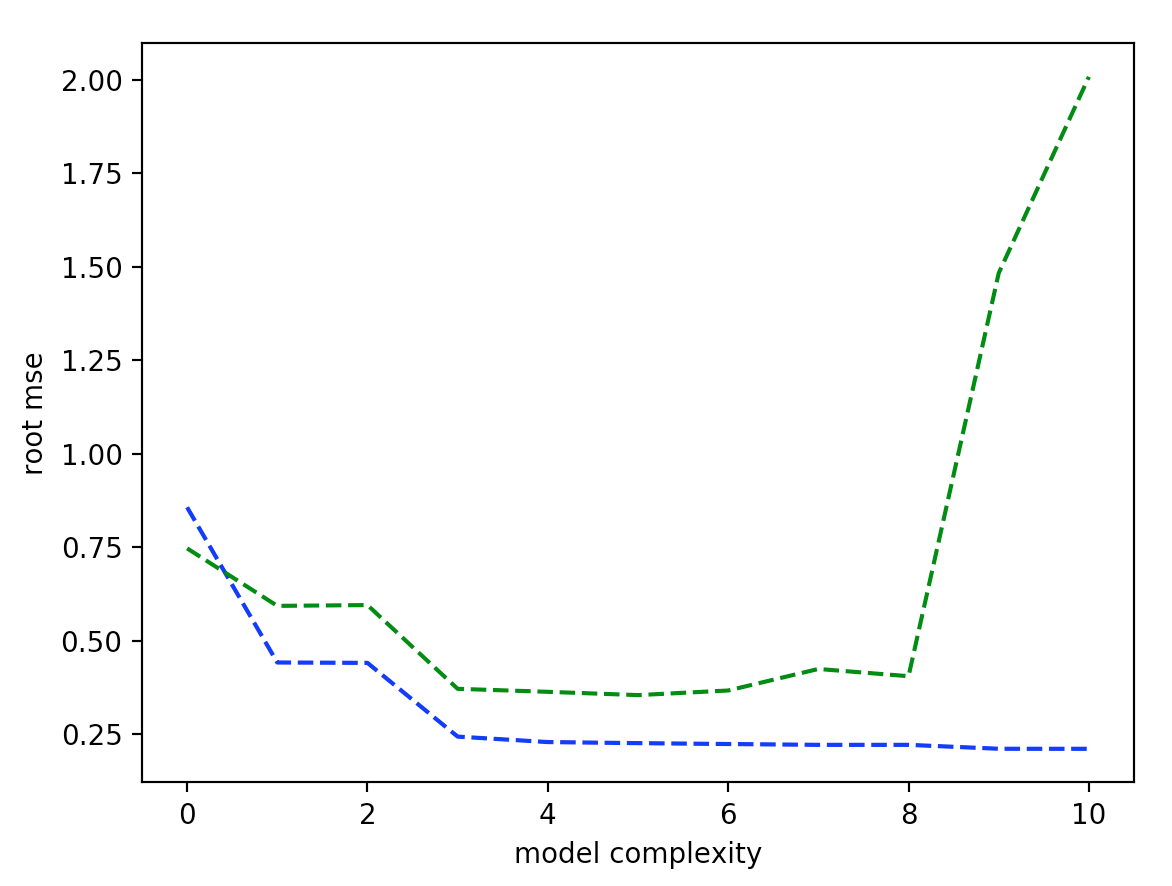
\includegraphics[scale=0.5]{ps111.png}
\newline{}
The green plot indicates test error, the blue plot indicates training error (not sure why matplotlib didn't show it). The best model complexity is a degree 8 polynomial. There is overfitting after degree 8 since training error continues to decrease but test error goes up quickly. 
\end{enumerate}

\newpage
\section{Problem 2}

\solution{Solution to problem 2}
\newpage
\end{document}
